\chapter{Enhancement nel dominio spaziale}
In questo capitolo vediamo le principali tecniche di enhancement nel dominio dello spazio,ovvero modificando il valore dei pixel attraverso funzioni che prendono in input uno o più pixel dell'immagine che intendiamo trasformare.

Dividiamo il tipo di funzione che applichiamo all'immagine a seconda degli argomenti che prende in input:
\begin{description}
	\item[Trasformazioni puntuali] che operano pixel a pixel e sostanzialmente mappano i livelli di intensità in altri livelli;
	\item[Trasformazioni locali] prendono in input un pixel e i suoi vicine, sono quelle in assoluto più usate e sono chiamate \textbf{filtri};
	\item[Trasformazioni globali] prendono come argomento l'intera immagine, tipicamente non ci permettono di ottenere una nuova immagine, ma servono a estrarre informazioni globali sull'immagine.
\end{description}

\section{Trasformazioni puntuali}
Anche se queste funzioni permettono semplicemente di rimappare il livello di intensità pixel a pixel sono molto utili per ottenere immagini più ricche di informazione e correggere eventuali errori dovuti all'acquisizione o allo strumento di visualizzazione dell'immagine.

Sono inoltre queste trasformazioni che ci permettono di ottenere immagini in pseudocolori o in falsi colori. Queste trasformazioni sono particolarmente utili in ambito medico e scientifico, dove è necessario evidenziare dettagli su immagini ottenute attraveso sensori che catturano fenomeni non osservabili otticamente.
\subsection{Look Up Table}
\begin{wrapfigure}{r}{.4\linewidth}
	\vspace{-.6cm}
	\centering
	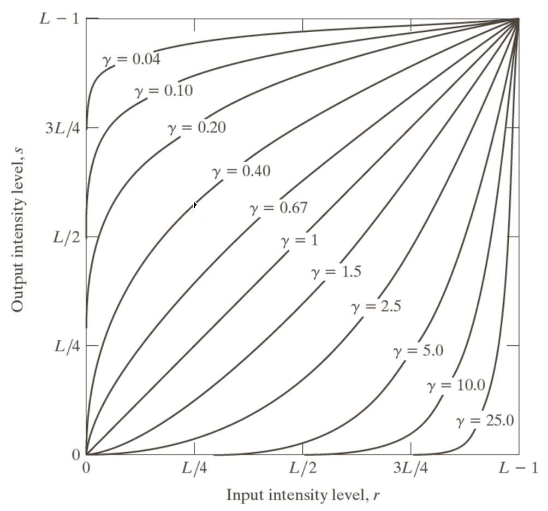
\includegraphics[width=.9\linewidth]{Picture/Gamma_Trasformation}
\end{wrapfigure}
I metodi che prevedono una funzione per rimappare i livelli di grigio solitamente si basano su Look Up Table (\textbf{LUT}) che specificano per ogni livello di grigio in ingresso il nuovo livello di grigio del pixel in uscita. Nell'immagine si può vedere una tipica trasformazione generata con una Power-Law, questa trasformazione serviva per correggere la gamma dei televisori a tubo catodico e prende quindi il nome di \textbf{gamma correction}.

\subsubsection{Tipologie di LUT}
Non c'è nessuna regola sul come costruire una LUT per rimappare i livelli di grigio, a seconda dell'obbiettivo che si vuole raggiungere si può costruire la LUT più adatta. Vediamo alcune tipologie particolarmente importanti:
\begin{itemize}
	\item \textbf{scala}: serve per ridurre il numero di livelli di grigio, opera una compressione lossy e può generare falsi bordi;
	\item \textbf{rampa}: serve per incrementare il contrasto in una particolare regione, ovviamente se si incrementa da una parte si riduce al di fuori della rampa;
	\item \textbf{binario}: permette di binarizzare l'immagine mettendo al massimo i livelli in un certo range e tutti gli altri a zero.
	\item \textbf{pseudocolor}: permette di colorare un'immagine in scala di grigi, consiste in realtà in tre diverse LUT che permettono di ottenere ciascuna una diversa componente RGB
\end{itemize}

\subsection{Bit-plane slicing}
\begin{wrapfigure}[7]{r}{.55\linewidth}
	\vspace{-.6cm}
	\centering
	\includegraphics[width=.95\linewidth]{Picture/Bit_slicing}
\end{wrapfigure}
Questa trasformazione permette di ottenere sempre immagini binarizzate. Per fare questo consideriamo l'immagine suddivisa in livelli, se la profondità colore è 8 ci saranno 8 livelli e il terzo sarà costituito da tutti i bit in terza posizione. Se consideriamo solo un livello otteniamo l'immagine binarizzata, possiamo poi unire diversi livelli assieme.

A seconda di che livello consideriamo possiamo ottenere differenti informazioni, perfino il livello associato al bit meno significativo (che genera un immagine apparentemente solo rumorosa) può portare informazioni utili, oppure può permette di inserire informazioni utili non visibili come watermark.

\section{Trasformazioni globali}
Permettono di ottenere informazioni utili sull'immagine e usarle per migliorare difetti tipici quali la sotto/sovra esposizione o basso contrasto.

\subsection{Istogramma}
Un indicatore molto utilizzato nelle trasformazioni globali è l'istogramma, che permette di ottenere la distribuzione in frequenza dei vari livelli di grigio di un'immagine.

\begin{wrapfigure}[7]{r}{.45\linewidth}
	\vspace{-.6cm}
	\centering
	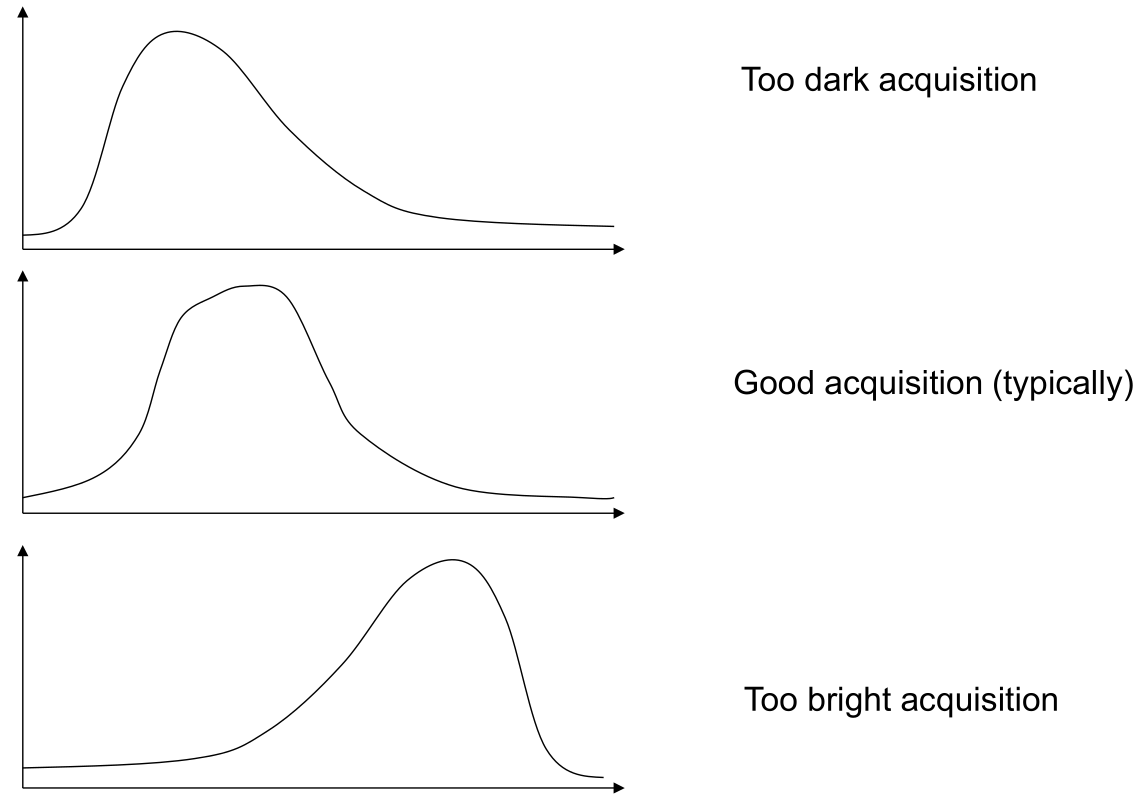
\includegraphics[width=.85\linewidth]{Picture/Histogram_Example}
\end{wrapfigure}
Semplicemente guardando la forma dell'istogramma ci si può rendere conto della bontà dell'immagine, o per lo meno della corretta esposizione. In un'immagine ci aspettiamo una distribuzione normale dai vari livelli di grigio, con pochi pixel che saturano il sensore in alto o in basso.

\begin{wrapfigure}[14]{l}{.4\linewidth}
	\vspace{-.3cm}
	\centering
	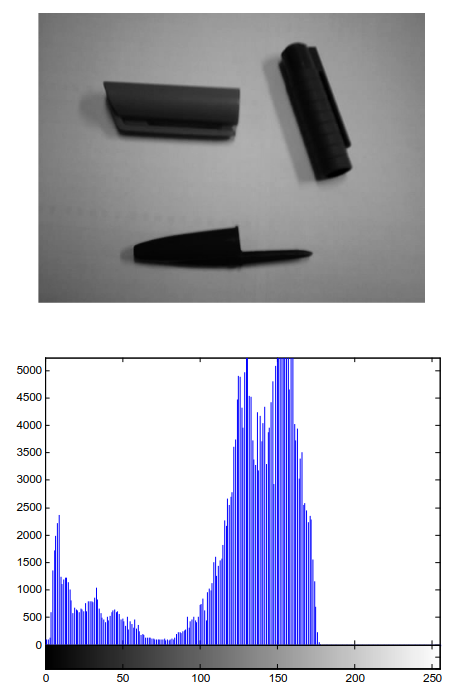
\includegraphics[width=.85\linewidth]{Picture/Histogram_Threshold}
\end{wrapfigure}
L'istogramma può inoltre essere utile per stimare la soglia di threshold più adatta a binarizzare un'immagine, infatti se siamo di fronte a un istogramma bimodale possiamo essere ragionevolmente certi che un picco rappresenti lo sfondo , mentre l'altro gli oggetti di nostro interesse. Tipicamente questa situazione si ritrova nei contesti di visione industriale e raramente nelle immagini naturali. Nell'immagine vediamo una situazione in cui è particolarmente evidente il valore che ci permette di avere una binarizzazione ragionevole dell'immagine; siamo quindi in una situazione molto favorevole.

\subsubsection{Equalizzazione dell'istogramma}
Una volta ottenuto l'istogramma di un immagine si può tentare di equalizzarlo in modo da migliorare l'immagine. Un istogramma concentrato solo su alcuni valori fa perdere dinamicità all'immagine, può quindi avere senso cercare di ripristinare una distribuzione uniforme dei valori dei pixel. Alla fine dell'equalizzazione vorremmo essere in una situazione come quella mostrata in figura qui sotto.

\begin{wrapfigure}[19]{r}{.45\linewidth}
	\vspace{-.4cm}
	\centering
	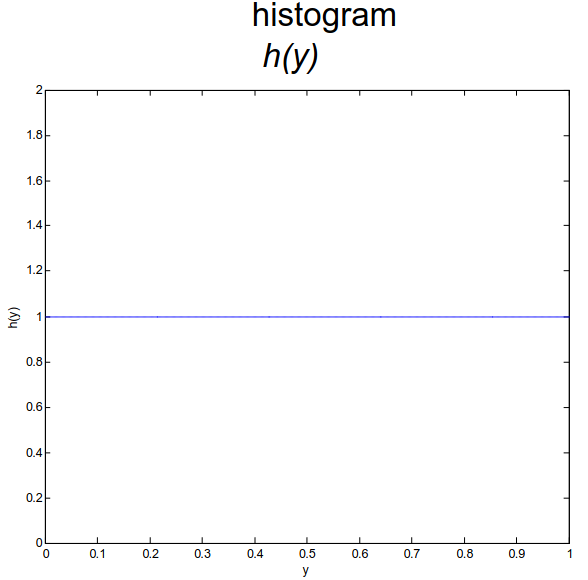
\includegraphics[width=.9\linewidth]{Picture/Histogram_EQ1}
	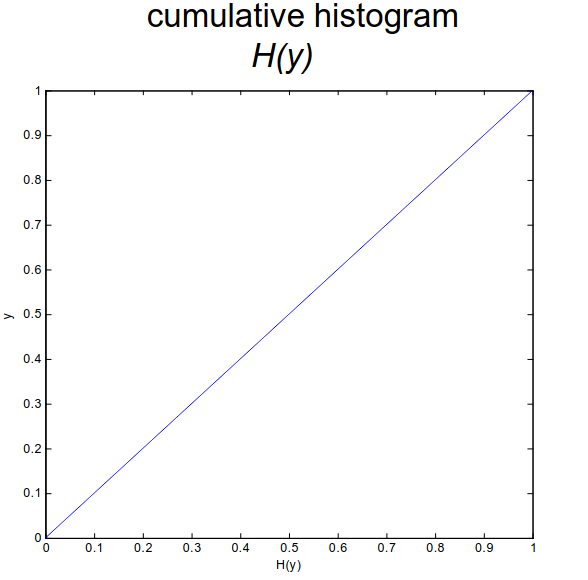
\includegraphics[width=.9\linewidth]{Picture/Histogram_EQ2}
\end{wrapfigure}
Per ottenere questo risultato consideriamo l'istogramma dell'immagine: $h(r)$ che associa a ogni livello di grigio $r$ il numero di pixel con quel valore. Definiamo l'istogramma cumulativo
\begin{equation}
	H(r) = \sum_{i = 0}^{r} h(i)
\end{equation}
e la funzione di trasformazione
\begin{equation}
	T(r) = (L - 1) \cdot \frac{H(r)}{M \cdot N}
\end{equation}
Dove $L$ è il numero di livelli di grigio, e $M$ e $N$ sono le dimensioni dell'immagine. Infine per ottenere l'immagine equalizzata trasformiamo ciascun pixel con
\begin{equation}
	y(i,j) = T[x(i,j)]
\end{equation}
Applicando queste trasformazioni possiamo ottenere un immagine con un istogramma equalizzato. È possibile che diversi livelli di grigio dell'immagine di partenza vengano mappati nello stesso livello di grigio dell'immagine di arrivo, è quindi necessari prestare attenzione alla possibile perdita di informazioni.

Si può costruire una trasformazione anche per ottenere una nuova immagine con un istogramma specificato, non per forza con distribuzione uniforme. Per fare questo costruisce $T$ che equalizza l'immagine di partenza, $G$ che equalizza l'istogramma che vogliamo ottenere, infine la trasformazione che permette di ottenere l'istogramma voluto sarà $z = G^{-1}(T(r))$.
\pagebreak
\section{Filtri}
\subsection{Caratteristiche generali}
I filtri permettono di applicare modifiche locali all'immagine e possono essere progettati sia nel dominio dello spazio che della frequenza. In questa prima e più semplice trattazione ci concentriamo sui filtri nel dominio dello spazio, indagando come certe caratteristiche dell'immagine possano essere messe in evidenza o nascoste a seconda di come progettiamo il filtro.

I filtri sono trasformazioni locali che si basano sulla \textbf{convoluzione} fra i pixel dell'immagine e una matrice che rappresenta il filtro stesso. Ci occuperemo di filtri:
\begin{itemize}
	\item Spazio invarianti;
	\item Lineari.
\end{itemize}
Date queste caratteristiche possiamo studiare l'effetto di un filtro semplicemente osservando la \textbf{risposta all'impulso}.  Siccome progetteremo sempre filtri 2D simmetrici fare la convoluzione sarà equivalente a sovrapporre la matrice quadrata che rappresenta il filtro all'immagine, moltiplicare i pixel per i pesi corrispondenti, sommare i risultati e immagazzinare il nuovo valore nel pixel centrale.

\subsection{Filtri passa-basso}
I filtri passa basso come suggerito dal nome sono filtri che eliminano le componenti a frequenza più alta, cioè si concentrano sui bordi dell'immagine sfumandoli.
\subsubsection{Media mobile}
\begin{wrapfigure}{r}{.5\linewidth}
	\vspace{-.3cm}
	\centering
	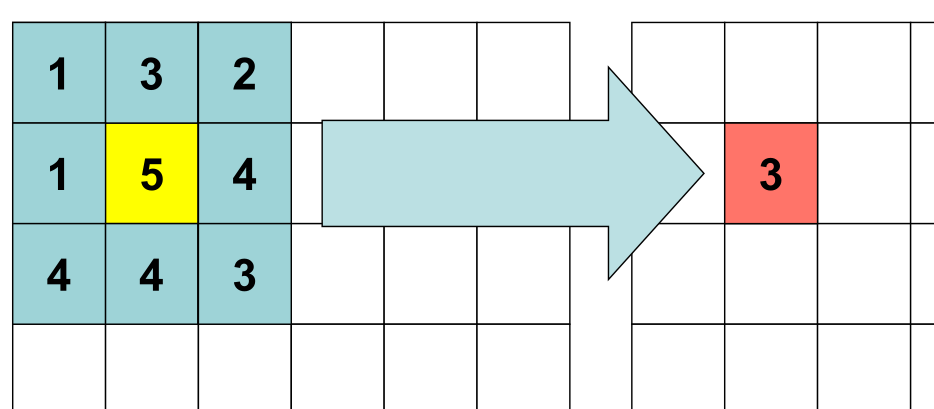
\includegraphics[width=.9\linewidth]{Picture/Moving_Average}
\end{wrapfigure}
Il più semplice filtro passa-basso e la media mobile, consiste nello scegliere una certa dimensione del filtro (\textbf{finestra}) e fare la media di tutti i pixel che si trovano nella finestra. Vedremo che un approccio di questo tipo può generare artefatti quando progetteremo filtri nel dominio della frequenza \ref{asd}.
\pagebreak
\subsubsection{Mediana}
\begin{wrapfigure}{l}{.6\linewidth}
	\centering
	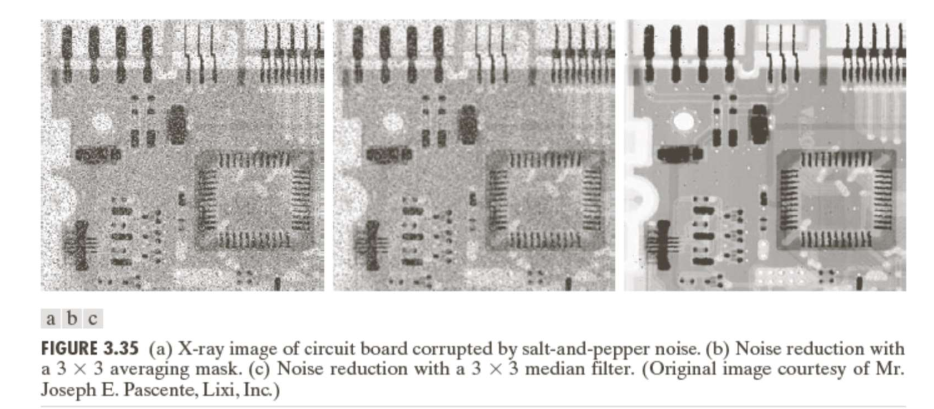
\includegraphics[width=.95\linewidth]{Picture/Median_Filter}
\end{wrapfigure}
Questo è un filtro non lineare, dato che la funzione che applica non è lineare, è comunque in filtro interessante dato che fa una statistica dei pixel all'interno della finestra e prende la mediana tra i pixel. Per questa ragione riesce a eliminare gli outlier che potrebbero essere presenti. Si comporta particolarmente bene per la rimozione del rumore sale e pepe.

\subsection{Filtri passa-alto}
I filtri passa alto servono per aumentare la nitidezza dell'immagine (\textbf{sharpening}) ed estrarre i bordi. Si ottengono cercando di calcolare le derivate dell'immagine, basandosi sull'idea che nei pressi dei bordi la derivata sarà elevata dato che c'è un cambio repentino nel valore dei pixel.
\subsubsection{Istogramma}
Prima di progettare dei filtri ad hoc proviamo ad applicare strumenti gia visti per aumentare il contrasto lungo i bordi. Possiamo ridefinire il concetto di equalizzazione in modo locale, andando considerare l'immagine costituita da sotto-immagini e equalizzando ciascuna parte in modo indipendente. Questo permette di aumentare il contrasto solo di alcune zone, ad esempio confrontando il valore medio dei pixel della zona con il valore medio dei pixel dell'immagine intera.
\subsubsection{Derivata dell'immagine}
Consideriamo la coordinata $x$ e definiamo la derivata nel caso discreto semplicemente come la differenza tra un campione e il successivo.
\begin{equation}
	\frac{\partial f}{\partial x} = f(x+1) - f(x)
\end{equation}
Data questa definizione possiamo applicare l'operatore derivata (che è lineare) alla derivata prima e ottenere la derivata seconda
\begin{equation}
	\frac{\partial^2 f}{\partial x^2} = f(x+1) + f(x-1) - 2 \cdot f(x)
\end{equation}
\subsubsection{Laplaciano}
Usando la derivata seconda possiamo costruire l'operatore laplaciano, questo operatore è invariante per rotazione e permette di aumentare la nitidezza dell'immagine.
\begin{wrapfigure}[14]{r}{.26\linewidth}
	\vspace{-.4cm}
	\centering
	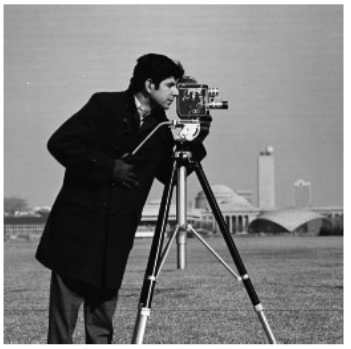
\includegraphics[width=.9\linewidth]{Picture/Cameraman_Original}
	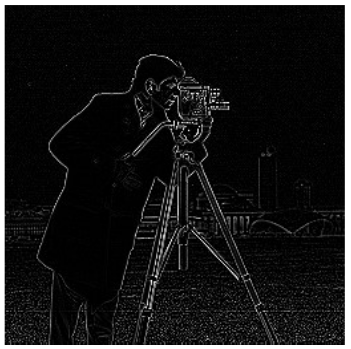
\includegraphics[width=.9\linewidth]{Picture/Cameraman_Laplacian}
\end{wrapfigure}
Definiamo il laplaciano come:
\begin{equation}
	\nabla^2 f = \frac{\partial^2 f}{\partial x^2} +  \frac{\partial^2 f}{\partial y^2}
\end{equation}
Possiamo ottenere un'immagine più nitida applicando la trasformazione
\begin{equation}
	g(x,y) = f(x,y) + c\cdot \nabla^2 f(x,y)
\end{equation}
Dove $c$ è un parametro che normalmente vale $\pm 1$.

Nell'immagine si vede il risultato del laplaciano applicato all'immagine (non è stato fatto sharpening, è solo stato applicato l'operatore $\nabla ^2$).
\subsubsection{Gradiente}
Considerando la derivata prima possiamo definire il gradiente dell'immagine in un dato pixel. Il gradiente è un vettore con una sua direzione e modulo. Possiamo usare il gradiente per costruire filtri che mettano in evidenza i bordi dell; immagine, dato che il gradiente ha una direzione possiamo considerare solo alcune componenti per enfatizzare i bordi orizzontali, verticali od obliqui; Oppure possiamo sommare tutte le componenti per evidenziare tutti i bordi.
\begin{wrapfigure}[7]{l}{.26\linewidth}
	\vspace{-.4cm}
	\centering
	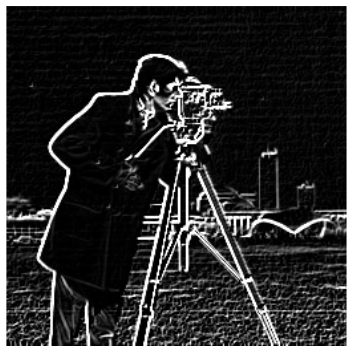
\includegraphics[width=.9\linewidth]{Picture/Cameraman_Gradient}
\end{wrapfigure}
Il gradiente è definito come:
\begin{equation}
	\nabla f = \frac{\partial f}{\partial x} \vec{i} +  \frac{\partial^2 f}{\partial y^2} \vec{j}
\end{equation}
Ed è sempre ortogonale alla direzione dei bordi dell'immagine. Se consideriamo solo le componenti orizzontali o verticali possiamo costruire gli operatori di Sobel mostrati qui sotto.
\begin{equation}
	S_x = 
	\begin{bmatrix}
		-1 & -2 & -1 \\
		0 & 0 & 0 \\
		1 & 2 & 1 
	\end{bmatrix}
	\quad \quad \quad
	S_y = 
	\begin{bmatrix}
		-1 & 0 & 1 \\
		-2 & 0 & 2\\
		-1 & 0 & 1 
	\end{bmatrix}
\end{equation}
L'immagine di esempio è stata ottenuta sommando il risultato dei due operatori di Sobel che evidenziano rispettivamente bordi orizzontali e verticali.

\section{Combinare gli strumenti}
Tutti gli strumenti presentati possono essere applicati in cascata per ottenere l'immagine desiderata. Ogni trasformazione ha lo scopo di semplificare il lavoro degli operatori a valle.
\begin{center}
	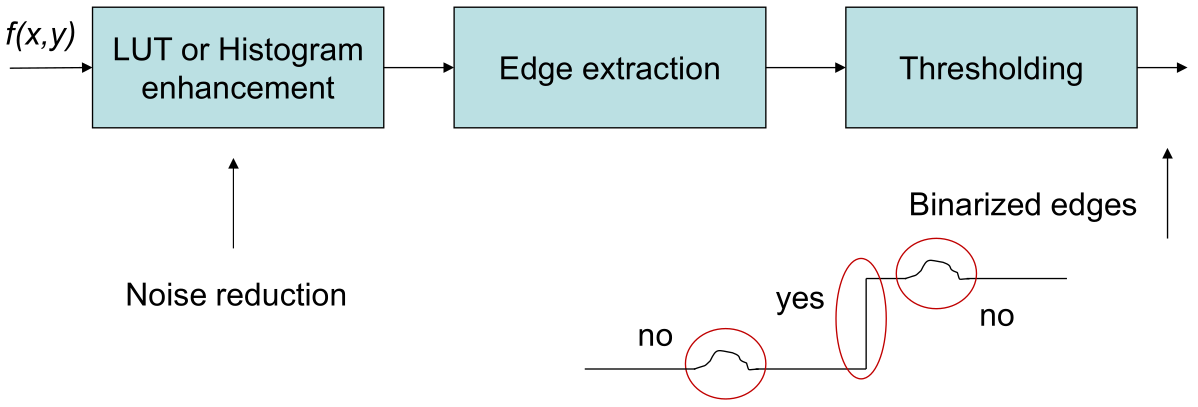
\includegraphics[width=.9\linewidth]{Picture/Enhancement_Pipeline}
\end{center}
Nell'immagine si vede una tipica pipeline di elaborazione di un'immagine, ovviamente ogni passaggio è optional e la sua applicazione o meno dipende dall'immagine di partenza, ma soprattutto dal risultato che si vuole ottenere; ricordando che l'enhancement è application-driven.